 \documentclass[12pt,letterpaper]{article}

\usepackage{multicol}
\usepackage[x11names,table]{xcolor}
\usepackage{pstricks}
\usepackage{marginnote}
\usepackage[shortlabels]{enumitem}

\usepackage{parskip}
\usepackage{times}

%Configuracion del la hoja

\usepackage{geometry} %Paquete de margenes
\geometry{left=4cm, right=3cm, top=3cm, bottom=3cm}% Tamaño del área de escritura de la páginas
\usepackage{lscape}


%Paquetes para el entorno de escritura
\usepackage[spanish]{babel}
\usepackage[utf8]{inputenc} %Reconoce tildes y otros simbolos propios del español
\setlength\parindent{12pt}
\usepackage[breaklinks=true, hidelinks]{hyperref}


%Paquetes necesarios en el entorno cientifico
\usepackage{amsmath} %Paquete de smbología matemática de la American Mathematical Society.
\usepackage{amsfonts}%Paquete de smbología matemática de la American Mathematical Society.
\usepackage{amssymb}
\usepackage{latexsym}
\usepackage{graphicx} % Required for the inclusion of images
\usepackage{subfigure} % subfiguras
%\usepackage{circuitikz} % Requerido para dibujar circuitos
%\usepackage{tikz}
%\usepackage{siunitx} % Provides the \SI{}{} and \si{} command for typesetting SI units

%Paquetes para herramientas útiles en el desarrollo del texto
\usepackage{float}%Requerido para obligar a los elementos a colocarse donde uno quiera
\usepackage[final]{pdfpages} % util para agregar pdf al final del documento

%Paquetes para la bibliografia
\usepackage{natbib} % Requerido para cambiar bibliografia a formato APA
%\usepackage{cite}	
\usepackage{listings}


\renewcommand{\labelenumi}{\alph{enumi}.} % Make numbering in the enumerate environment by letter rather than number (e.g. section 6)

\newcommand{\newfig}[4]{%
\begin{figure}[H]%
\centering%
\includegraphics[width=#1\linewidth]{#2}%
\caption{\emph{\small{#3}}}%
\label{fig:#4}
\end{figure}%
}

\usepackage{pgfgantt} %Cronograma de actividades

%----------------------------------------------------------------------------------------
%	PRESENTACION DEL DOCUMENTO
%----------------------------------------------------------------------------------------



\author{} % Author name

\date{FECHA} % Date for the report

\begin{document}

\renewcommand{\listfigurename}{Lista de Figuras}
\renewcommand{\listtablename}{Lista de Tablas}
\renewcommand{\contentsname}{Lista de Contenidos}
\renewcommand{\figurename}{Figura}
\renewcommand{\tablename}{Tabla}


% Insert the title, author and date
\begin{center}

	\vspace{3cm} ANTEPROYECTO \\

	\vspace{8cm} DISEÑO DE UN SENSOR INTELIGENTE PARA LA MEDICIÓN DE VARIABLES AMBIENTALES Y MECÁNICAS PARA APLICACIONES DE MONITOREO DE SALUD ESTRUCTURAL
\end{center}


\vspace{6cm}

\begin{flushleft}
	TUTOR ACADÉMICO: José Romero \\
\end{flushleft}


\begin{flushright}

	Presentado ante la ilustre\\
	Universidad Central de Venezuela\\
	por el BR. Jose Alejandro Tovar Briceño \\
	para optar por el título de \\
	Ingeniero Electricista   \\

\end{flushright}


\vspace{2cm}
\thispagestyle{empty}
\newpage


\begin{center}
	\section*{ INTRODUCCIÓN}
\end{center}

La seguridad en la construcción de infraestructuras es un tema de gran importancia en la actualidad, especialmente cuando se trata de estructuras críticas como edificios o puentes.

Los primeros indicios del monitoreo del estado de las infraestructuras data de nuestro comienzos como especie sedentaria.  En la antigüedad, los constructores utilizaban técnicas de inspección visual y auditiva para detectar posibles problemas en las estructuras, como grietas o ruidos inusuales. Con el tiempo, se desarrollaron técnicas más avanzadas para el monitoreo de estructuras, como la utilización de medidores de deformación y sensores de vibración.

La integración de la instrumentación con el análisis estructural comenzó a desarrollarse en la década de 1960 con el advenimiento de la informática y la disponibilidad de computadoras capaces de realizar cálculos estructurales complejos. En esa época, se comenzaron a utilizar sistemas de medición de datos para recopilar información sobre el comportamiento de las estructuras en tiempo real y utilizarla para calibrar y validar los modelos estructurales.

Actualmente, las normas sismoresistentes apuntan a estructuras que sean capaces de mantener su integridad ante un evento de esta magnitud. Además, el monitoreo continuo de la salud estructural permite evaluar el comportamiento de la estructura en caso de sismo y validar los modelos estructurales utilizados en la normativa sismorresistente. Para el monitoreo a largo plazo, el resultado de este proceso es información actualizada periódicamente sobre la capacidad de la estructura para desempeñar su función prevista a la luz del inevitable envejecimiento y degradación resultantes de los entornos operativos.

%Incluir conjunto de elementos que influyen en el deterioro de la estructura. Envejecimiento, mantenimiento

En este sentido, el monitoreo de las estructuras se ha convertido en una herramienta esencial para garantizar la seguridad de las personas en caso de sismos y cumplir con las normas sismorresistentes. Además, el monitoreo de las estructuras puede ayudar a mejorar la eficacia de las normas sismorresistentes, ya que permite validar y mejorar los modelos estructurales utilizados en la normativa.

Para garantizar la seguridad de estas estructuras, es necesario contar con sistemas de monitoreo que permitan detectar posibles daños o fallas en su funcionamiento y tomar medidas preventivas. Por tanto, los sistemas de adquisición de datos y monitoreo son herramientas esenciales en la prevención de accidentes y daños.

En este trabajo de grado se abordará el diseño para una futura implementación de un sistema de adquisición de datos inalámbrico de bajo costo basado en un microcontrolador para el monitoreo de variables como aceleración, inclinación, humedad y temperatura en estructuras críticas, con el objetivo de prevenir daños y accidentes en estas estructuras.


%Además de poder monitorear y realizar acciones sobre los sistemas, los instrumentos de medida de última tecnología se fabrican de modo que puedan ser compatibles con medios de comunicación inalámbricas lo que posibilita la transmisión de datos adquiridos sin necesidad de cable a la central del sistema \textit{SCADA}. El presente trabajo de grado pretende realizar el diseño de un sistema de adquisición y transmisión de datos integrando microcontroladores ESP32 a medidores de energía eléctrica para formar una red mallada inalámbrica capaz de transmitir los datos recolectados a un punto central.

\newpage



\begin{center}
	\section*{ PLANTEAMIENTO DEL PROBLEMA}
\end{center}


\vspace{0.3cm}

La seguridad en las estructuras es un tema crítico en la ingeniería, especialmente en lo que respecta a estructuras críticas como edificios y puentes. A medida que el tiempo pasa, estas estructuras pueden deteriorarse y presentar fallas que pueden poner en riesgo la vida de las personas que las utilizan. Por lo tanto, es fundamental contar con sistemas de monitoreo que permitan detectar posibles problemas en las estructuras y tomar medidas preventivas.

Sin embargo, la mayoría de los sistemas de monitoreo de estructuras disponibles en el mercado son costosos y no están diseñados específicamente para aplicaciones de salud estructural. Además, muchos de estos sistemas no tienen capacidad para admitir comunicación inalámbrica, lo que limita su aplicación en estructuras de gran tamaño o en áreas de difícil acceso, además de los costos asociados a un sistema de cableado fiable que no perturbe las mediciones.


%La energía eléctrica es diferente de otras manifestaciones de la energía, debido a que no se puede almacenar por si sola como electricidad. Esto obliga a que la energía eléctrica consumida por un equipo u aparato tenga que generarse al momento en el cual se vaya a consumir. Los procesos para la generación de energía tienen costos altos de desarrollo e implementación a gran escala (países o estados) por lo que surtir de energía a las industrias y electrodomésticos tiene un costo que la empresa que genera la energía necesita recuperar. Como consecuencia se suele medir el consumo de cada uno de los usuarios por razones enteramente económicas.\\


%En Venezuela se utiliza el mismo método de adquisición de datos desde que se instaló el sistema eléctrico. Este consiste en un operador que se acerca hasta el lugar donde se encuentra un medidor de energía y registra la lectura que marca el medidor, esto se hace de manera repetitiva para todos los sitios donde se quiera registrar el consumo. En ocasiones los medidores tienen una salida codificada donde comunica el valor del consumo por infrarrojo lo que permite al operador registrar el valor de ese consumo mediante un aparato compatible con este protocolo. Debido a esta problemática surge la necesidad de sustituir este sistema de adquisición de datos manual por uno que no requiera el traslado del operador hasta el sitio, que sea económico, confiable y eficiente.\\


%Los principales equipos de medición de energía poseen en su diseño una salida por pulsos y soportan distintos protocolos de comunicación, lo que representa una ventaja al trabajar con microcontroladores, pues estos son adaptables a la mayoría de los protocolos mediante programación lo que facilita la adquisición de los datos a partir del medidor. Por otra parte trabajar con microcontroladores ofrece la posibilidad de realizar comunicaciones inalámbricas si se adapta un módulo WiFi como periférico. Interconectar estos módulos WiFi para formar una red mallada permitiría la transmisión de los datos captados a una mayor distancia que la lograda por un único módulo y permitiría su salida hacia alguna red externa deseada sin utilizar cables entre los medidores y la central de adquisición de datos, y sin intervención presencial del operador. Ilustradas las debilidades expuestas anteriormente y las ventajas que representaría un sistema de este tipo se evidencia la necesidad de realizar el diseño.\\



\newpage


\begin{center}
	\section*{JUSTIFICACIÓN}
\end{center}

\vspace{1cm}


Un sensor inteligente que conste de un sistema de adquisición de datos basado en un microcontrolador que recolecte y procese la información adquirida en conjunto con varios sensores dispuestos en un solo dispositivo permite realizar la medición de variables ambientales y mecánicas de interés en aplicaciones de salud estructural a un bajo costo; además, un sistema de este tipo es flexible en cuanto a las variables a medir puesto que es compatible con distintos tipos de sensores y a los métodos de comunicación a utilizarse, permitiendo crear soluciones canalizadas a proyectos en específico, logrando disminuir costos y contribuir de una forma más eficaz al proceso de toma de decisiones estructurales.

Existe variedad en cuanto al hardware de bajo costo que puede utilizarse para la implementación de un prototipo del sistema, lo que ofrece un alternativa atractiva a los sistemas de adquisición actuales, además de la capacidad de transmisión que ofrecen las redes de larga distancia disponibles en conjunto con las capacidades de los microcontroladores, permitiendo que la estación base pueda ubicarse lejos de la estructura crítica.

Para lograr medir todas estas variables en tiempo real es conveniente contar con un microcontrolador capaz de manejar toda esta información sin dejar de lado la fiablidad en la adquisición de estos datos y que su vez sea capaz de emplear las herramientas necesarias para comunicar estos datos de forma inalámbrica.

Sabiendo esto, existe una necesidad clara de desarrollar un sistema de adquisición de datos y monitoreo inalámbrico y de bajo costo para aplicaciones de salud estructural con capacidad de admitir comunicación inalámbrica que permita detectar posibles fallas en las estructuras y tomar medidas preventivas para garantizar la seguridad de las personas.


\newpage


\begin{center}
	\section*{ANTECEDENTES}
\end{center}

\vspace{1cm}

La implementación de microcontroladores para sistemas de adquisición de datos es un tema que se ha desarrollado en múltiples aplicaciones. Muchas veces, se logran desarrollar soluciones que permiten disminuir costos sin que eso afecte la calidad de las mediciones. Las soluciones que se tomarán como referencia lograron: Desarrollar sistemas de adquisición de datos basados en microcontroladores para la medición de variables físicas. Además, se han logrado crear redes de sensores inteligentes que permiten facilitar el envío de los datos de forma inalámbrica.

%El concepto de una red mallada no es algo nuevo, consiste en una serie de dispositivos conectados todos entre sí con la capacidad de comunicarse y enviar datos a un lugar de destino. Las soluciones ya existentes que se tomarán como referencia han logrado: utilizar redes malladas de sensores que permiten una recolección y trasmisión de datos fuera de la red. Ademas se ha logrado comunicar de manera inalámbrica a dispositivos que originalmente no poseen esa facultad, equipando estos aparatos con módulos WiFi y un microcontrolador para el manejo del envío y recepción. Los trabajos mencionados se presentan a continuación:\\


El trabajo de \cite{federici2014design} en \textit{"Design of Wireless Sensor Nodes for Structural Health Monitoring applications"} publicado en Procedia Engineering. Este trabajo aborda el diseño de redes de sensores inalámbricos para la monitorización del estado de estructuras civiles, centrándose específicamente en el diseño de nodos en relación con los requisitos de diferentes clases de aplicaciones de monitorización estructural.
Los problemas de diseño se analizan con referencia específica a una configuración experimental a gran escala (la monitorización estructural a largo plazo de la Basílica S. Maria di Collemaggio, L'Aquila, Italia). Se destacan las principales limitaciones que surgieron y se esbozan las estrategias de solución adoptadas, tanto en el caso de la plataforma de detección comercial como de las soluciones totalmente personalizadas. Se revisan las opciones para el diseño y despliegue del sistema de monitorización, tanto en el caso de la selección de plataformas comerciales como en el caso del desarrollo de plataformas a la medida.

En cuanto al desarrollo realizado por \cite{komarizadehasl2022development} en \textit{"Development of Low-Cost Sensors for Structural Health Monitoring Applications"}, el ingeniero Komarizadehasl propone cuatro sistemas de monitorización de alta precisión y bajo coste.
En primer lugar, para medir correctamente las respuestas estructurales, se desarrolla el Cost Hyper-Efficient Arduino Product (CHEAP). CHEAP es un sistema compuesto por cinco acelerómetros sincronizados de bajo coste conectados a un microcontrolador Arduino que hace el papel de dispositivo de recogida de datos. Para validar su rendimiento, se efectuaron unos experimentos de laboratorio y sus resultados se compararon con los de dos acelerómetros de alta precisión (PCB393A03 y PCB 356B18). Se concluye que CHEAP puede usarse para Monitoreo de Salud Estructural en estructuras convencionales con frecuencias naturales bajas cuando se cuente con presupuestos de monitoreo escasos. 

En segundo lugar, se presenta un inclinómetro de bajo coste, un Low-cost Adaptable Reliable Angle-meter (LARA), que mide la inclinación mediante la fusión de distintos sensores: cinco giroscopios y cinco acelerómetros. LARA combina un microcontrolador basado en la tecnología del Internet de las Cosas (NODEMCU), que permite la transmisión inalámbrica de datos, y un software comercial gratuito para la recogida de datos (SerialPlot). Para confirmar la precisión y resolución de este dispositivo, se compararon sus mediciones en condiciones de laboratorio con las teóricas y con las de un inclinómetro comercial (HI-INC). Los resultados de laboratorio de una prueba de carga en una viga demuestran la notable precisión de LARA. Se concluye que la precisión de LARA es suficiente para su aplicación en la detección de daños en puentes.

En tercer lugar, también se dilucida el efecto de la combinación de sensores de rango similar para investigar el aumento de la precisión y la mitigación de los ruidos ambientales. Para investigar la teoría de la combinación de sensores, el ingeniero Komarizadehasl, propone un equipo de medición compuesto por 75 sensores para la medición de distancias acoplados a dos microcontroladores de Arduino. Los 75 sensores son 25 HC-SR04 (analógicos), 25 VL53L0X (digitales) y 25 VL53L1X (digitales). Los resultados muestran que promediando la salida de varios sensores sin calibrar, la precisión en la estimación de distancia aumenta considerablemente.

El último sistema propuesto por Komarizadehasl presenta un novedoso y versátil sistema de adquisición de datos a distancia que permite el registro del tiempo con una resolución de microsegundos para la sincronización posterior de las lecturas de los sensores inalámbricos situados en diversos puntos de una estructura. Esta funcionalidad es lo que permitiría su aplicación a pruebas de carga estáticas o quasi-estaticas o al análisis modal de las estructuras.


\cite{muttillo2019structural} en su trabajo \textit{"Structural health continuous monitoring of buildings - A modal parameters identification system"} propone en su tesis el diseño de un Sistema de Monitorización de la Salud Estructural (Structural Health Monitoring) para monitorizar y comprobar continuamente el comportamiento estructural a lo largo de la vida útil del edificio. El sistema, compuesto por un datalogger personalizado y dispositivos esclavos, permite la monitorización continua de la aceleración de la estructura gracias a su facilidad de instalación y bajo coste. El sistema propuesto se basa principalmente en un microcontrolador que: 

\begin{itemize}
	\item Se comunica con los nodos a través del bus RS485, 
	\item Sincroniza las muestras de adquisición
	\item Adquiere los datos medidos por los nodos.
\end{itemize} 

El sistema fue probado en una estructura de aluminio en voladizo, a través de tres campañas experimentales diferentes y los datos medidos, recogidos en una memoria interna del datalogger, fueron post-procesados a través del algoritmo Matlab. Los resultados permitieron evaluar con éxito los parámetros modales (frecuencias, amortiguamiento y formas modales) de la estructura analizada y su estado de salud.

%\cite{QCGJ2018} en su trabajo ”Sistema De Monitoreo de Variables Medioambientales Usando Una Red de Sensores Inalámbricos y Plataformas De Internet De Las Cosas” se pensó en un sistema para la recolección de datos meteorológicos usando una red de sensores inalámbricos (RSI), capaz de transmitir datos en tiempo real. El sistema logró automatizar procesos de obtención de datos de manera continua y a largo plazo, por medio de un módulo de abastecimiento de energía solar que permite autonomía para su funcionamiento. Se propuso la utilización de dos sistemas: DigiMesh y WiFi. El procesamiento se realizó en un Arduino Uno, para la comunicación se utilizó un XBee PRO 900HP (DigiMesh) y un moduló Electric Imp.01 (WiFi). Adicionalmente se evaluó la transmisión de los datos hacia plataformas de Internet de las cosas (IoT), en donde se gestionará y visualizará los datos obtenidos por los nodos. Este sistema fue pensado como alternativa de bajo costo para sistemas meteorológicos y está basado en componentes de hardware y software libre. Al realizarse la validación de los datos obtenidos mediante un análisis estadístico con los datos registrados por una estación meteorológica se obtuvo un error relativo promedio máximo de 4,93 \%.\\


\newpage


\begin{center}
	\section*{OBJETIVOS}
\end{center}

\vspace{1cm}

\subsection*{OBJETIVO GENERAL}

Diseñar un sensor inteligente para la medición de variables ambientales y mecánicas para aplicaciones de Monitoreo de Salud Estructural.

\subsection*{OBJETIVOS ESPECÍFICOS}


\begin{enumerate}[1.]


	\item Documentar las principales características y la importancia del monitoreo para aplicaciones de salud estructural.

	\item Documentar los principales métodos de recolección de datos soportados por los sensores necesarios para la medición de las variables de interés.

	\item Evaluar y proponer el protocolo de comunicación que permita el envío fiable de los datos recolectados por el sensor inteligente.

	\item Seleccionar el hardware adecuado tanto sensores como microcontrolador para la implementación futura del sistema.

	\item Diseñar el módulo de programa encargado de la recolección y almacenamiento de los datos provenientes de los sensores.

	\item Desarrollar el módulo de programa encargado de la comunicación de los datos usando la tecnología escogida.

	\item Validar el funcionamiento del sistema haciendo uso de un prototipo de pruebas.

\end{enumerate}
\newpage



\begin{center}

	\section*{ MARCO METODOLÓGICO}

\end{center}

\vspace{1cm}

Con la finalidad de realizar efectivamente cada objetivo del proyecto, se llevará a cabo la siguiente metodología:
\bigskip

\begin{enumerate}[1.]



	\item Documentar las principales características y la importancia del monitoreo para aplicaciones de salud estructural.

	      \begin{enumerate}

		      \item Investigación documental acerca de los principales métodos de extracción de datos soportados por los sensores de interés.

		      \item Comparación de los métodos para extracción de datos desde un sensor según las ventajas que ofrecen al usar un microcontrolador.

		      \item Selección del método de extracción de datos a ser utilizado en el sistema con miras a su posterior procesamiento y envío.


	      \end{enumerate}

	\item  Documentar los principales métodos de recolección de datos soportados por los sensores necesarios para la medición de las variables de interés.


	      \begin{enumerate}

		      \item Investigación documental sobre el hardware disponible en el mercado capaz de realizar las actividades previstas.

		      \item Comparación entre sensores para cada una de las variables de interés.

		      \item Comparación entre microcontroladores con base en la naturaleza de los sensores, su método de comunicación y su adaptabilidad al sistema

		      \item Selección del hardware a utilizarse en el prototipo.



	      \end{enumerate}


	\item Evaluar y proponer el protocolo de comunicación que permita el envío fiable de los datos recolectados por el sensor inteligente.

	      \begin{enumerate}

		      \item Investigación documental sobre los protocolos de comunicación disponibles según el microcontrolador y el hardware de comunicaciones a utilizarse.

		      \item Comparación entre las distintas opciones.

		      \item Selección del método de comunicación y del hardware necesario para el envío y recepción de datos.

	      \end{enumerate}


	\item Seleccionar el hardware adecuado tanto sensores como microcontrolador para la implementación futura del sistema.


	      \begin{enumerate}

		      \item Programación para el manejo del hardware externo al microcontrolador, capaz de recibir datos de señales analógicas y digitales.
		      \item Adquisición de datos de variables físicas.
		      \item Almacenamiento de los datos en memoria no volátil.

	      \end{enumerate}

	\item Diseñar el módulo de programa encargado de la recolección y almacenamiento de los datos provenientes de los sensores.


	      \begin{enumerate}

		      \item Programación para el manejo del hardware capaz de enviar los datos recolectados y manejo de la interfaz con el microcontrolador.
		      \item Envío de datos en tiempo real.

	      \end{enumerate}



	\item Desarrollar el módulo de programa encargado de la comunicación de los datos usando la tecnología escogida.


	      \begin{enumerate}

		      \item Montaje de prototipo tomando en cuenta consideraciones de ruido y acondicionamiento de señales.

	      \end{enumerate}

	\item Validar el funcionamiento del sistema haciendo uso de un prototipo de pruebas.


	      \begin{enumerate}

		      \item Pruebas para comprobar el funcionamiento del sistema de adquisición.
		      \item Pruebas para comprobar la comunicación hacia la estación base.
		      \item Comprobación de la calidad de los datos extraídos.

	      \end{enumerate}





\end{enumerate}




\newpage


\begin{center}

	\section*{ ALCANCE Y LIMITACIONES}
\end{center}

Los principales equipos de medición estructural cuentan con salidas digitales o en su defecto salidas analógicas que pueden ser convertidas y soportan distintos protocolos de comunicación, lo que representa una ventaja al trabajar con microcontroladores, pues estos son adaptables a la mayoría de los protocolos lo que facilita la adquisición de los datos a partir del medidor.

Los desafíos al usar el ADC de un microcontrolador en mediciones estructurales pueden ser varios. Uno de los principales es la precisión de la medición, ya que el ADC puede presentar errores en la conversión analógico-digital. Además, la resolución del ADC puede limitar la precisión de las mediciones, lo que puede afectar la calidad de los datos obtenido, esto se verificará comparando los resultados obtenidos con datos .

Otro desafío importante es la velocidad de muestreo, ya que en aplicaciones estructurales puede ser necesario tomar mediciones en tiempo real para detectar posibles fallas o cambios en el comportamiento de la estructura. En este sentido, es importante que el ADC del microcontrolador tenga una velocidad de muestreo adecuada para las necesidades de la aplicación.

Para validar el funcionamiento del sistema diseñado se propondrá la realización un prototipo de pruebas para demostrar el desempeño del diseño.



% \begin{figure}[H]
% 	\centering
% 	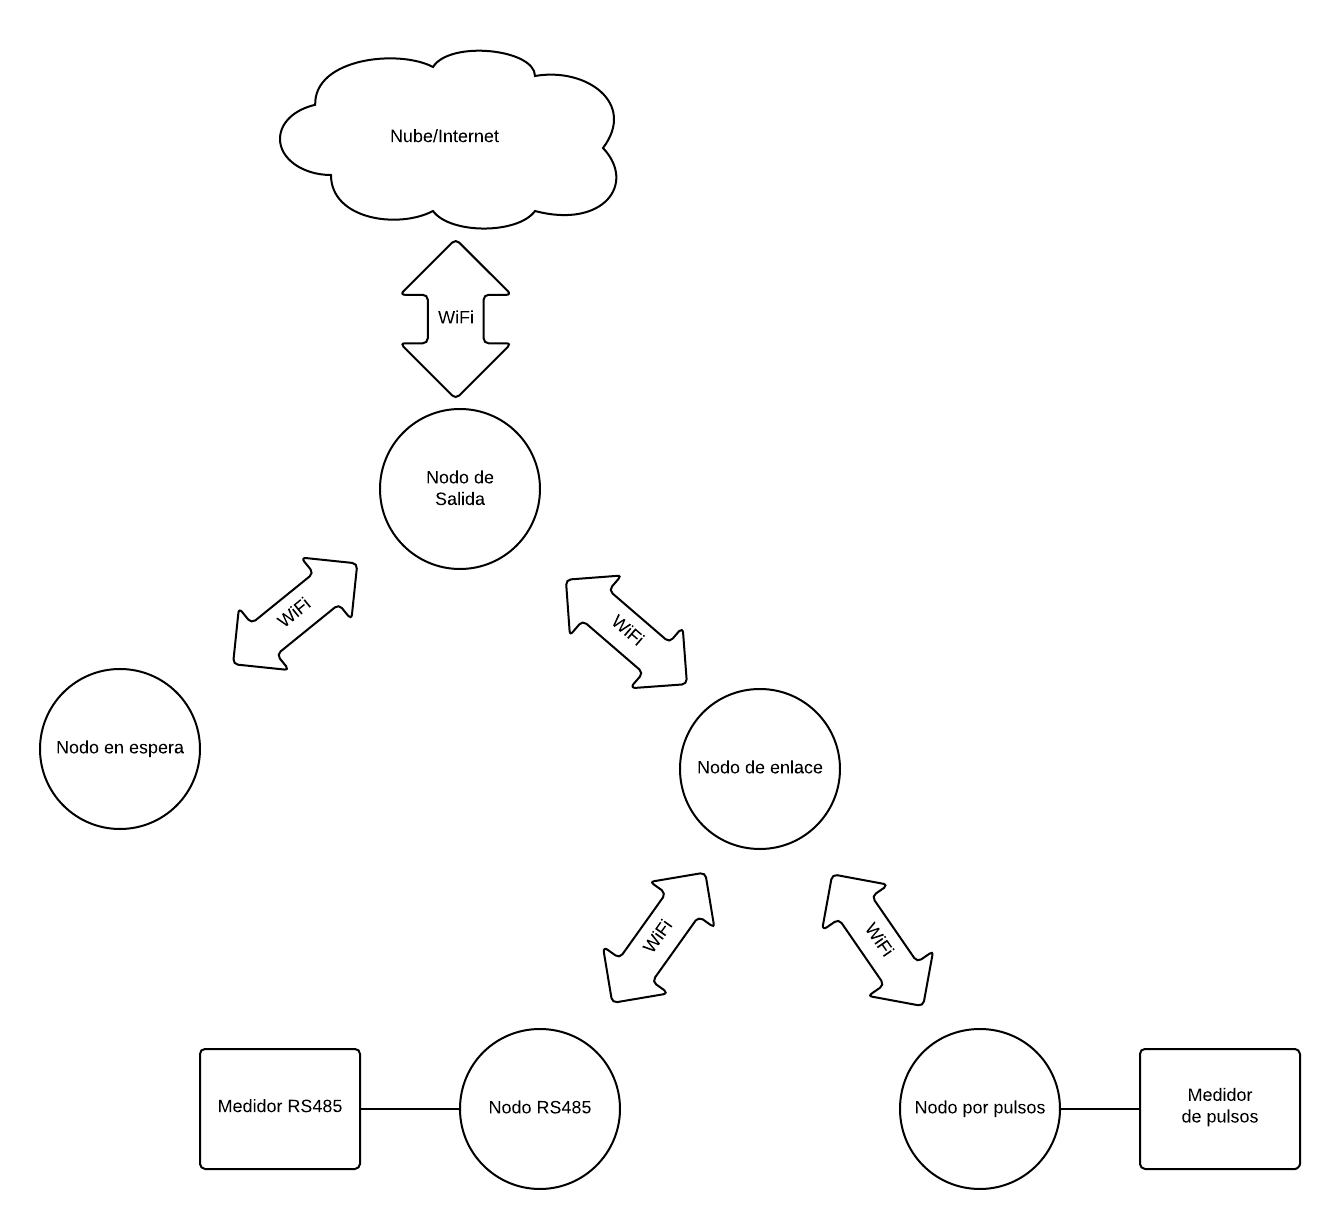
\includegraphics[width=0.7\linewidth]{EsquemaTEG.png}
% 	\caption{Representación gráfica de la red descrita en el alcance.}
% 	\label{fig:esquemateg}
% \end{figure}

%\newfig{0.7}{imagenes/EsquemaTEG.png}{Representación gráfica de la red descrita en el alcance. PRUEBA}{esquemateg}

\newpage

\begin{center}
	\section*{ RECURSOS Y FACTIBILIDAD}
\end{center}

Para el desarrollo e implementación del sistema se requiere de microcontroladores, sensores de aceleración, humedad, inclinación y temperatura, módulos de radiofrecuencia y un computador para la instalación del Interfaz de Desarrollo (IDE )necesario para el desarrollo de aplicaciones en el microcontrolador.

Tanto los microcontroladores como los módulos y sensores necesarios serán suministrados por el Instituto de Materiales y Modelos Estructurales (IMME). El IDE a utilizarse, en conjunto con los frameworks necesarios, se escogerán dependiendo del microcontrolador (MCU) escogido con base en la investigación a realizarse. El código estará disponible de forma libre en el manejador de versiones Github y contará con la documentación necesaria, escrita por los desarrolladores, para el correcto funcionamiento del sistema.

\newpage





\begin{center}

	\section*{ CRONOGRAMA DE ACTIVIDADES}



	\vspace{0.5cm}
	\resizebox{1.1\textwidth}{!}{
		\begin{ganttchart}[
				canvas/.append style={fill=none, draw=black!5, line width=.75pt},
				hgrid style/.style={draw=black!5, line width=.75pt},
				vgrid={*1{draw=black!5, line width=.75pt}},
				today label font=\small\bfseries,
				title/.style={draw=none, fill=none},
				title label font=\bfseries\footnotesize,
				title label node/.append style={below=6pt},
				include title in canvas=false,
				bar label font=\mdseries\small\color{black!70},
				bar label node/.append style={left=.3cm},
				bar/.append style={draw=none, fill=black!63},
				bar incomplete/.append style={fill=blue},
				bar progress label font=\mdseries\footnotesize\color{black!70},
				group incomplete/.append style={fill=blue},
				group left shift=0,
				group right shift=0,
				group height=.5,
				group peaks tip position=0,
				group label node/.append style={left=.3cm},
				group progress label font=\bfseries\small,
				link/.style={-latex, line width=1.5pt, red},
				link label font=\scriptsize\bfseries,
				link label node/.append style={below left=-2pt and 0pt},
			]{1}{24}
			\gantttitle{Diseñar un sensor inteligente para la medición de variables ambientales y mecánicas}{24} \\
			\gantttitle{para aplicaciones de Monitoreo de Salud Estructural}{24} \\[grid]
			\gantttitle[
				title label node/.append style={below left=7pt and -3pt}
			]{Semana:\quad1}{1}
			\gantttitlelist{2,...,24}{1} \\
			\ganttgroup{Documentar las aplicaciones de salud estructural}{1}{3} \\
			\ganttbar{\textbf{Investigación Documental}}{1}{1} \\
			\ganttbar{\textbf{Principales características de la salud estructural}}{2}{2} \\
			\ganttbar{\textbf{Importancia del monitoreo}}{3}{3} \\
			\ganttgroup{Documentar métodos de extracción}{4}{8} \\
			\ganttbar{\textbf{Investigación sobre sensores}}{4}{5} \\
			\ganttbar{\textbf{Compatibilidad con microcontroladores}}{5}{6} \\
			\ganttbar{\textbf{Características del Hardware}}{6}{8} \\
			\ganttgroup{Documentar y proponer el protocolo de comunicación}{9}{12} \\
			\ganttbar{\textbf{Investigación documental}}{9}{10} \\
			\ganttbar{\textbf{Compatibilidad con microcontroladores}}{10}{11} \\
			\ganttbar{\textbf{Manejo de buses}}{11}{12} \\
			\ganttgroup{Proponer el hardware necesario}{13}{16} \\
			\ganttbar{\textbf{Escoger microcontrolador}}{13}{15} \\
			\ganttbar{\textbf{Escoger sensores y hardware de comunicación}}{15}{16} \\
			\ganttgroup{Desarrollar módulo encargado de recolección de datos}{17}{20} \\
			\ganttbar{\textbf{Extracción fiable de las variables}}{17}{19} \\
			\ganttbar{\textbf{Almacenamiento en memoria}}{19}{20} \\
			\ganttgroup{Desarrollar módulo encargado de la comunicación}{21}{22} \\
			\ganttbar{\textbf{Comunicación interna y externa del sistema}}{21}{22} \\
			%\ganttbar{\textbf{Comunicación interna y externa de la red}}{23}{24} \\
			\ganttgroup{Validar funcionamiento}{22}{24} \\
			\ganttbar{\textbf{Montaje de prototipo}}{22}{23} \\
			\ganttbar{\textbf{Comparación con equipo de campo}}{23}{24} \\
		\end{ganttchart}
	}

\end{center}

\newpage

\bibliographystyle{apalike}

\bibliography{JT_Anteproyecto}

\end{document}

